\newpage
\section{Data from Nordark Work Packages}

This section holds infomation about data collected from the other workpackages in the Nordark project. The type of collected data/information is discussed against the possibility to visualize the data/information in the current version of the Digital Twin, as well as provides suggestions on possible future ways of using the DT for visualization.

\subsection{WP1: Analyzing the environmental psychology aspect} \label{env}

This section visualizes data coming from Work Package 1 regarding the environmental psychology aspect. The data is provided in teams group, named WP1-Ålesund data\_Day-Head torches.xlsx. The original data is in the excel format, as captured in Figure \ref{table} below. The answers were scaled from 1 to 5 and represented on the \textbf{Mean} column. \textbf{SD} stands for standard deviation.
\begin{figure}[H]
    \centering
    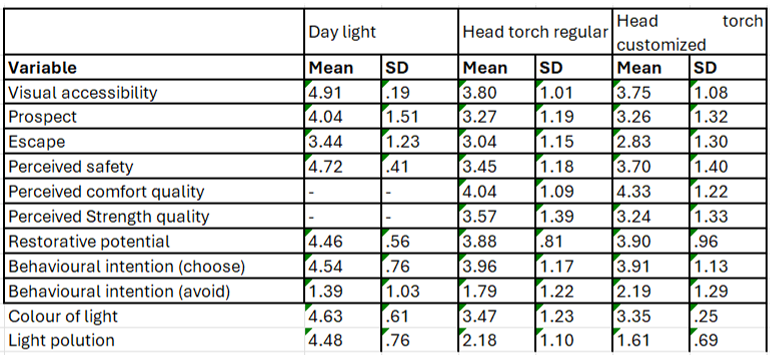
\includegraphics[width=0.8\textwidth]{Images/table.jpg}
    \caption[The original data from WP1 regarding the environmental psychology aspect]{The original data from WP1 regarding the environmental psychology aspect}
    \label{table}
\end{figure}

The goal of this survey is to assess pedestrian's satisfaction on three different conditions; (1) on the daylight, (2) using a regular head torch, and (3) using a cutomized head torch. The pedestrian's satisfaction was evaluated through several factors as listed on the \textbf{Variable} column on Figure \ref{table}. The dataset was gathered by surveying pedestrians as they walked along the selected path shown in Figure \ref{pedpath}. Data collection took place along the section of the path marked in red and yellow. Most responses were gathered around the midpoint of the stretch, where pedestrians first walked the path and then answered the questions while being immersed (half way).
\begin{figure}[H]
    \centering
    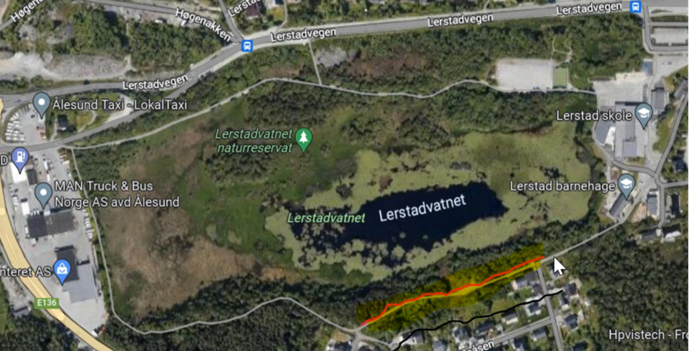
\includegraphics[width=0.75\textwidth]{Images/pedpath.jpg}
    \caption[The selected path to access the environmental psychology aspect]{The selected path to access the environmental psychology aspect}
    \label{pedpath}
\end{figure}

Given that the Nordark digital twin only supports geojson format on the data visualization feature, the original file needs to be converted to the geojson file. This new file is provided in teams group, named EnvironmentalPsychology.geojson. To meet the goal of this survey, we visualize the \textbf{Mean} of each condition and scale it between 0 to 1 in the heatmaped bar. To visualize the data on the digital twin, follow these steps:
\begin{itemize}
    \item Go to \textit{Data visualization} feature.
    \item Click the \textit{Add dataset} button, and select the file "EnvironmentalPsychology.geojson"
    \item Zoom out/in and adjust the camera to find the analyzed path
\end{itemize}

To illustrate the comparison on three different conditions, we visualized all three conditions in a single frame, as shown in Figure \ref{123}, where 1, 2, and 3 correspond to daylight, the regular head torch, and the customized head torch, respectively.
\begin{figure}[H]
    \centering
    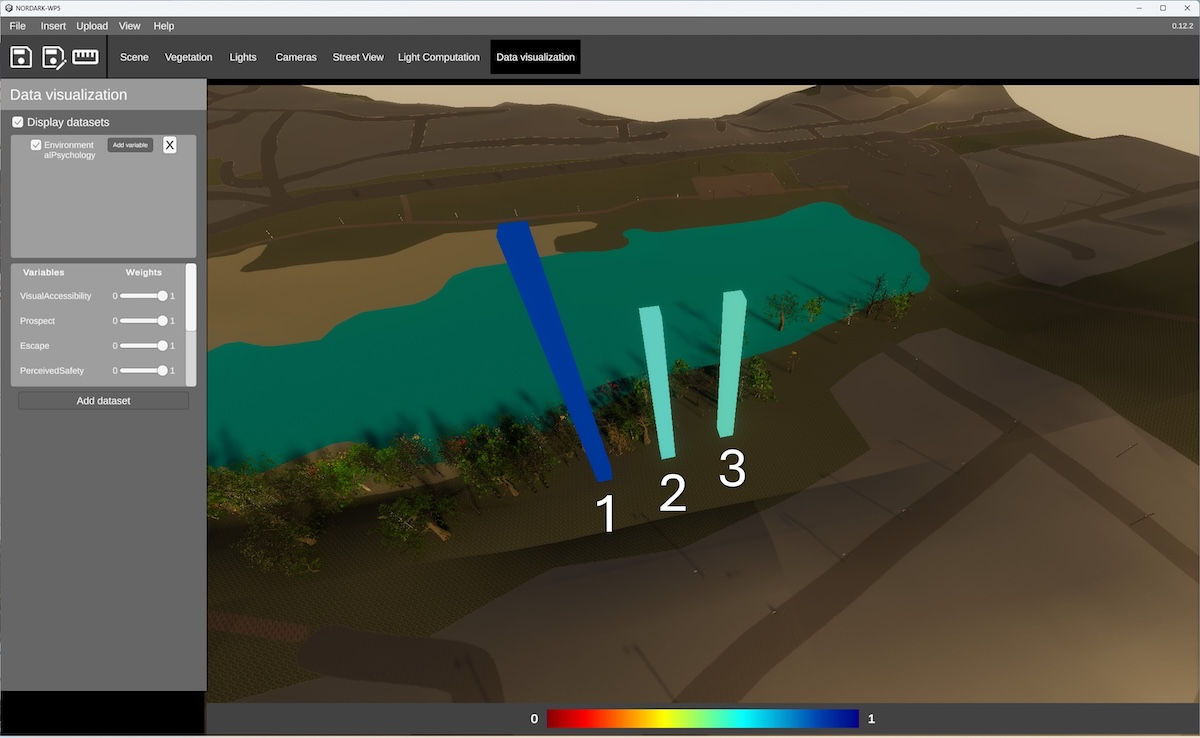
\includegraphics[width=0.75\textwidth]{Images/123.jpg}
    \caption[The analysis on the environmental psychology aspect]{The analysis on the environmental psychology aspect, 1 for day light, 2 for regular head torch, 3 for customized head torch.}
    \label{123}
\end{figure}

Figure \ref{pedestrian} presents the results for different setups of the analyzed variables. 0 in red indicates lower satisfaction levels, while 1 in blue represents the highest satisfaction. Part (a) of Figure \ref{pedestrian} considers only light polution factor. It shows that the pedestrians have lower satisfaction on the light polution produced by the customized head torch than the one from the regular head torch. On part (b) and (c), the pedestrians agreed that the customized head torch perceives a higher level of safety and comfort than the regular head torch.  As shown in parts (c) and (d), perceived comfort and strength qualities were not assessed under the daylight condition.
\begin{figure}[H]
    \centering
    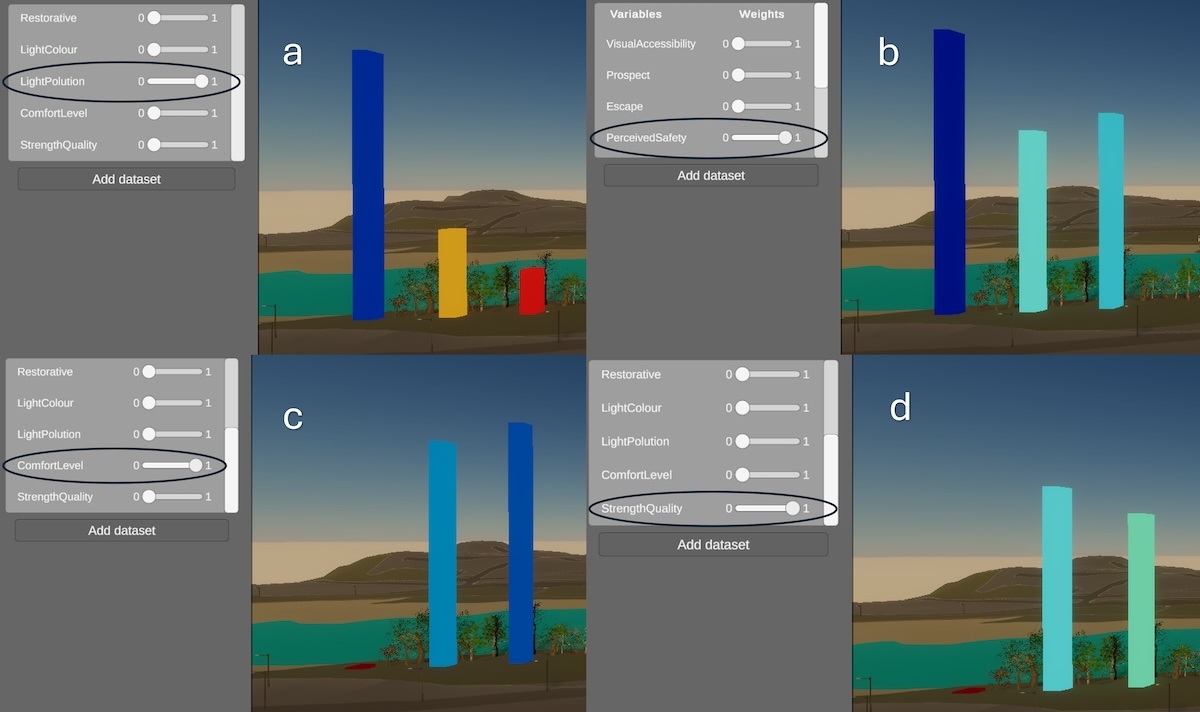
\includegraphics[width=0.9\textwidth]{Images/pedestrian.jpg}
    \caption[Data visualization on the environmental psychology aspect]{Data visualization on the environmental psychology aspect, (a) light polution, (b) perceived safety, (c) perceived comfort level, (d) perceived strength quality.}
    \label{pedestrian}
\end{figure}


\subsection{WP4: Comparing the measured data with the simulated data} \label{comparing}

This section covers data coming from Work Package 4 regarding the light measurement in Savja, Uppsala. This data is provided in teams group, named Light\_Data\_Uppsala\_WP5.xlsx. The light measurement was conducted on the location shown in Figure \ref{uppsala}
\begin{figure}[H]
    \centering
    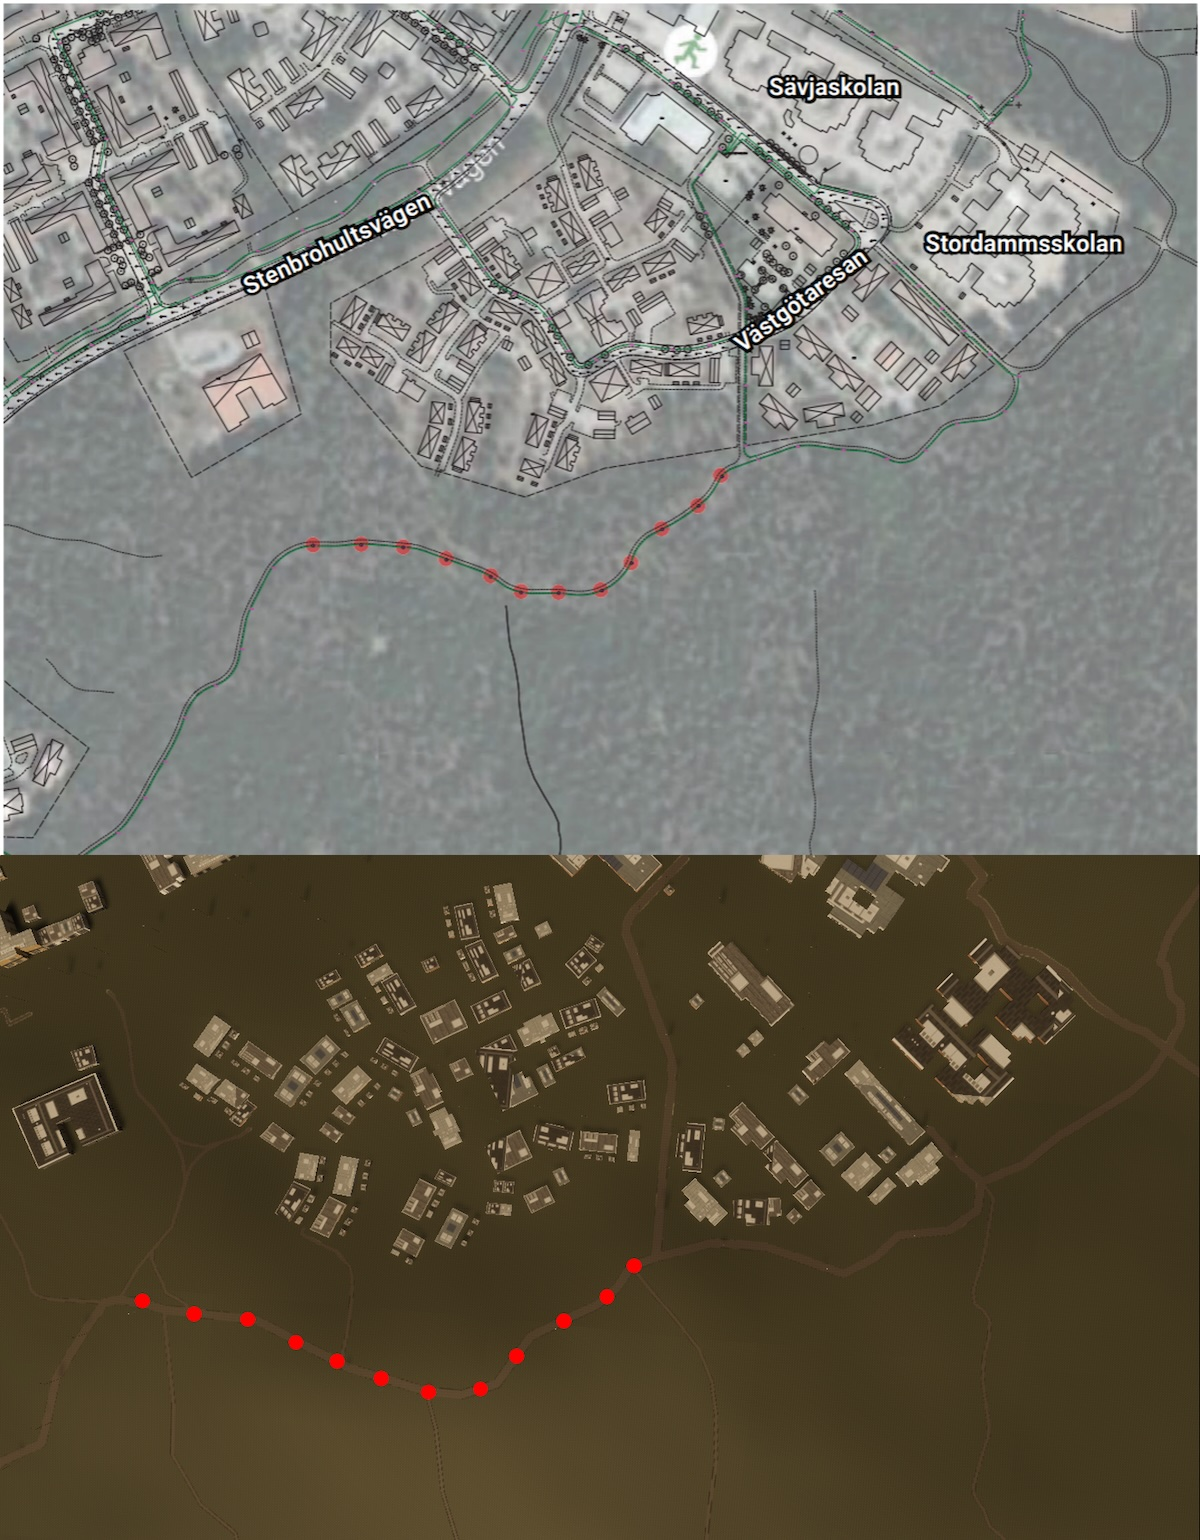
\includegraphics[width=0.7\textwidth]{Images/uppsala.jpg}
    \caption[The project location in Uppsala and chose light poles' positions for the field studies]{The project location in Uppsala and chose light poles' positions for the field studies. Top: a capture from Google Maps. Bottom: a capture from the digital twin software }
    \label{uppsala}
\end{figure}

The area between pole number 2 and 3 in Figure \ref{Savja} was selected as the main area of light measurements due to having a spacing of 30 metres, which represents the average spacing between poles on the walking route. By defaults, pole number 2 and 3 are identified as light 191 and 192, respectively, on the digital twin. 
\begin{figure}[H]
    \centering
    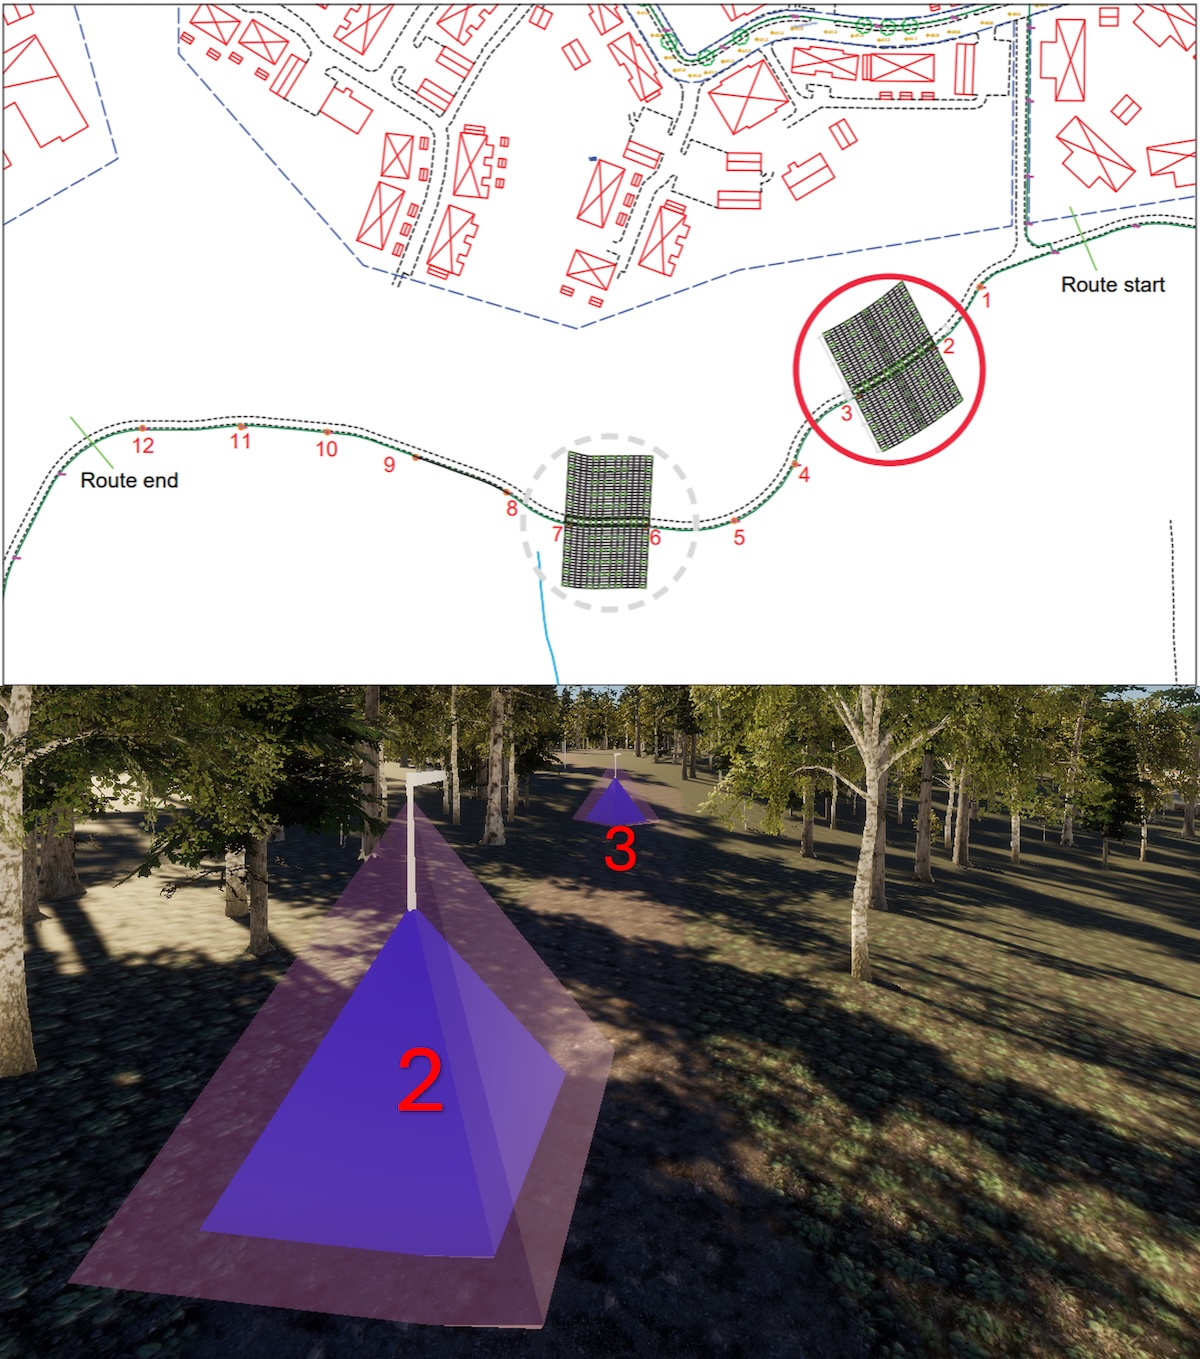
\includegraphics[width=0.7\textwidth]{Images/Savja.jpg}
    \caption[Area selected for the light measurements.]{Area selected for the light measurements. Top: full detailed measuremenets between poles 2 and 3, and control measurements between poles 6 and 7. Bottom: a capture from the digital twin software, showing poles 2 and 3.}
    \label{Savja}
\end{figure}

The grid for this light measurement is shown in Figure \ref{LM}. Since the light pole is needed as a starting point for drawing lines, we can only visualize the measured data that can be drawn horizontally and vertically from the light pole, which are illustrated as blue boxes in Figure \ref{LM}.
\begin{figure}[H]
    \centering
    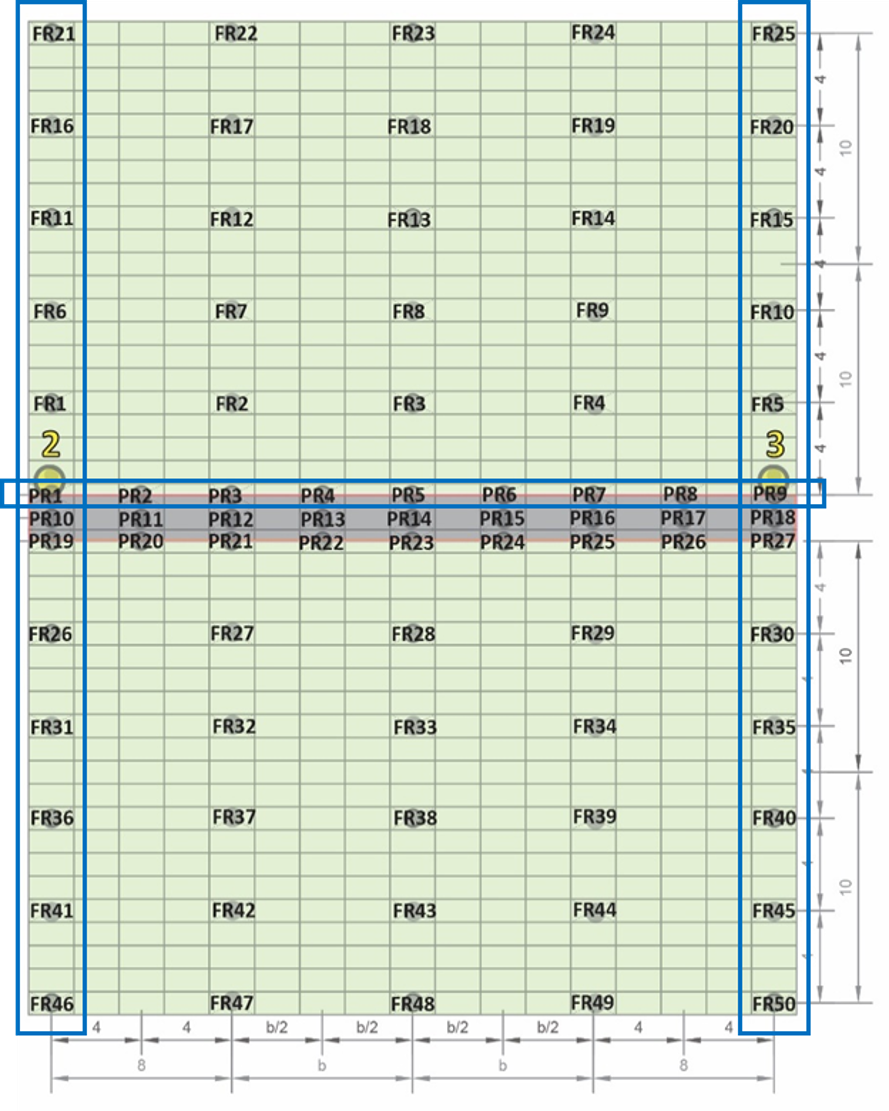
\includegraphics[width=0.7\textwidth]{Images/LM.jpg}
    \caption[The light measurement grid for poles 2 and 3]{The light measurement grid for poles 2 and 3}
    \label{LM}
\end{figure}

The Nordark digital twin only supports geojson format to be imported, therefore, the original data needs to be converted to the geojson file. One converted file is provided as an example, named case3.geojson. This file includes the measurement between light poles: PR1, PR2, PR3, PR4, PR5, PR6, PR7, and PR8. The case is intervention light measurements, Scenario 1 100\% (November - no snow) in Sävja, Uppsala - evening measurements - ground level (h: 0.00 m). To compare the measure data coming from WP4 and the modelled data on the digital twin, follow these steps: 
\begin{enumerate}
    \item Go to \textit{Scene} feature, change the location to Uppsala.    
    \item Go to \textit{Lights} feature, select the light poles 191 and 192, then change the IES file to \textit{Prisma Light Elton 1-S 830 DNW ROTERAD}. Note: by default, the first light pole you see on the Uppsala scene is light pole 195, to find light poles 191 and 192, you need to move forward. If you are not sure, you can use Figures \ref{uppsala} and \ref{Savja} to find the location of light poles 2 and 3 on the digital twin. 
    \item Go to \textit{Scene} feature, set the date to 17 November 2023, the time to 18:30, the clouds to Overcast.
    \item Go to \textit{Light computation} feature, click \textit{Create measure line around light pole} button, select "light 191", and set the parameter as shown in Figure \ref{drawline}, then click on \textit{Create measure line}.

    \begin{figure}[H]
    \centering
    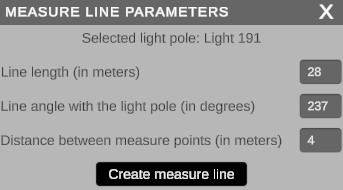
\includegraphics[width=0.4\textwidth]{Images/drawline.jpg}
    \caption[The measure line parameters for PR1 to PR8]{The measure line parameters for PR1 to PR8}
    \label{drawline}
    \end{figure}

    \item Go to \textit{Light computation} feature, check the \textit{Display graph} box to show the graph along the drawn line.
    \item Click the \textit{Import results} button, then select the case3.geojson file to import the light measurement data.
    \item if you follow all stages properly, from setting the scene, date, time, clouds, to finding the light pole and creating the exact line, then you will get the results as shown in Figure \ref{case3}.
\end{enumerate}

\begin{figure}[H]
    \centering
    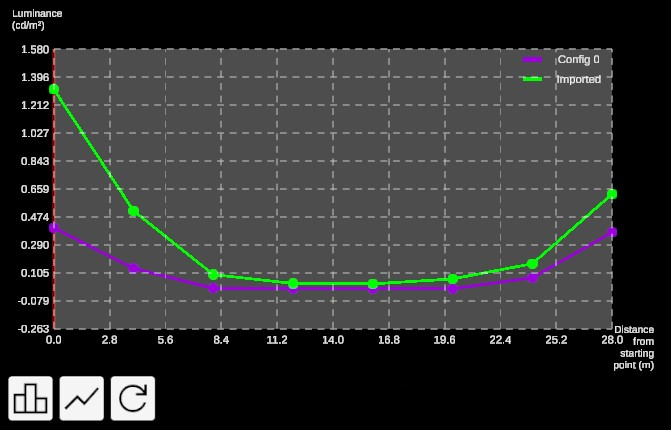
\includegraphics[width=0.8\textwidth]{Images/case3.jpg}
    \caption[The comparison of the measured data and the modelled data on PR1 to PR8, at 18:30 on 17 November 2023, no snow]{The comparison of the measured data and the modelled data on PR1 to PR8, at 18:30 on 17 November 2023, no snow. Purple line represents the modelled data, green line represents the measured data}
    \label{case3}
\end{figure}

The original light measurement data is provided in terms of illuminance (lux), whereas the digital twin system operates using luminance (lumen). To clarify the distinction between the two, as outlined in the \textit{Technical Documentation – NORDARK DT}:
\begin{itemize}
    \item Illuminance measures the amount of light being projected towards an object by the light (in lux).
    \item Luminance is the amount of light reflected off the surface being illuminated. It is considered the human perception of brightness.
\end{itemize}
In the digital twin, luminance is computed using color values and camera exposure. In a linear color space, the rendering-based formula is:
\begin{equation}
    Luminance = (0.0396819152, 0.458021790, 0.00609653955) * pixelColor / exposure 
\end{equation}
For converting measured illuminance data (lux) to luminance (cd/m²), a common approximation is:
\begin{equation}
    Luminance (cd/m2) = Illuminance (lux) * \rho / \pi
\end{equation}
where $\rho$ is reflectance of the surface. In the digital twin, the surface between light poles 2 and 3 is identified as an asphalt path, with a reflectance value of 0.05–0.15. While the surface around the trees is identified as forest, with a reflectance value of 0.1-0.2. Therefore, a reflectance value will be changed corresponding to the area surface.

To create a measurement line for the points PR1, PR10, PR19, FR26, FR31, FR36, FR41, and FR46, use the line parameters shown in Figure \ref{parameter}(a). For the points PR1, FR1, FR6, FR11, FR16, and FR21, refer to the parameters in Figure \ref{parameter}(b). Both of these lines should be assigned to light 191.

To create a measurement line for PR9, PR18, PR27, FR30, FR35, FR40, FR45, and FR50, use the parameters from Figure \ref{parameter}(c). For the line consisting of PR9, FR5, FR10, FR15, and FR22, use the parameters in Figure \ref{parameter}(d). These two lines should be associated with light 192.
\begin{figure}[H]
    \centering
    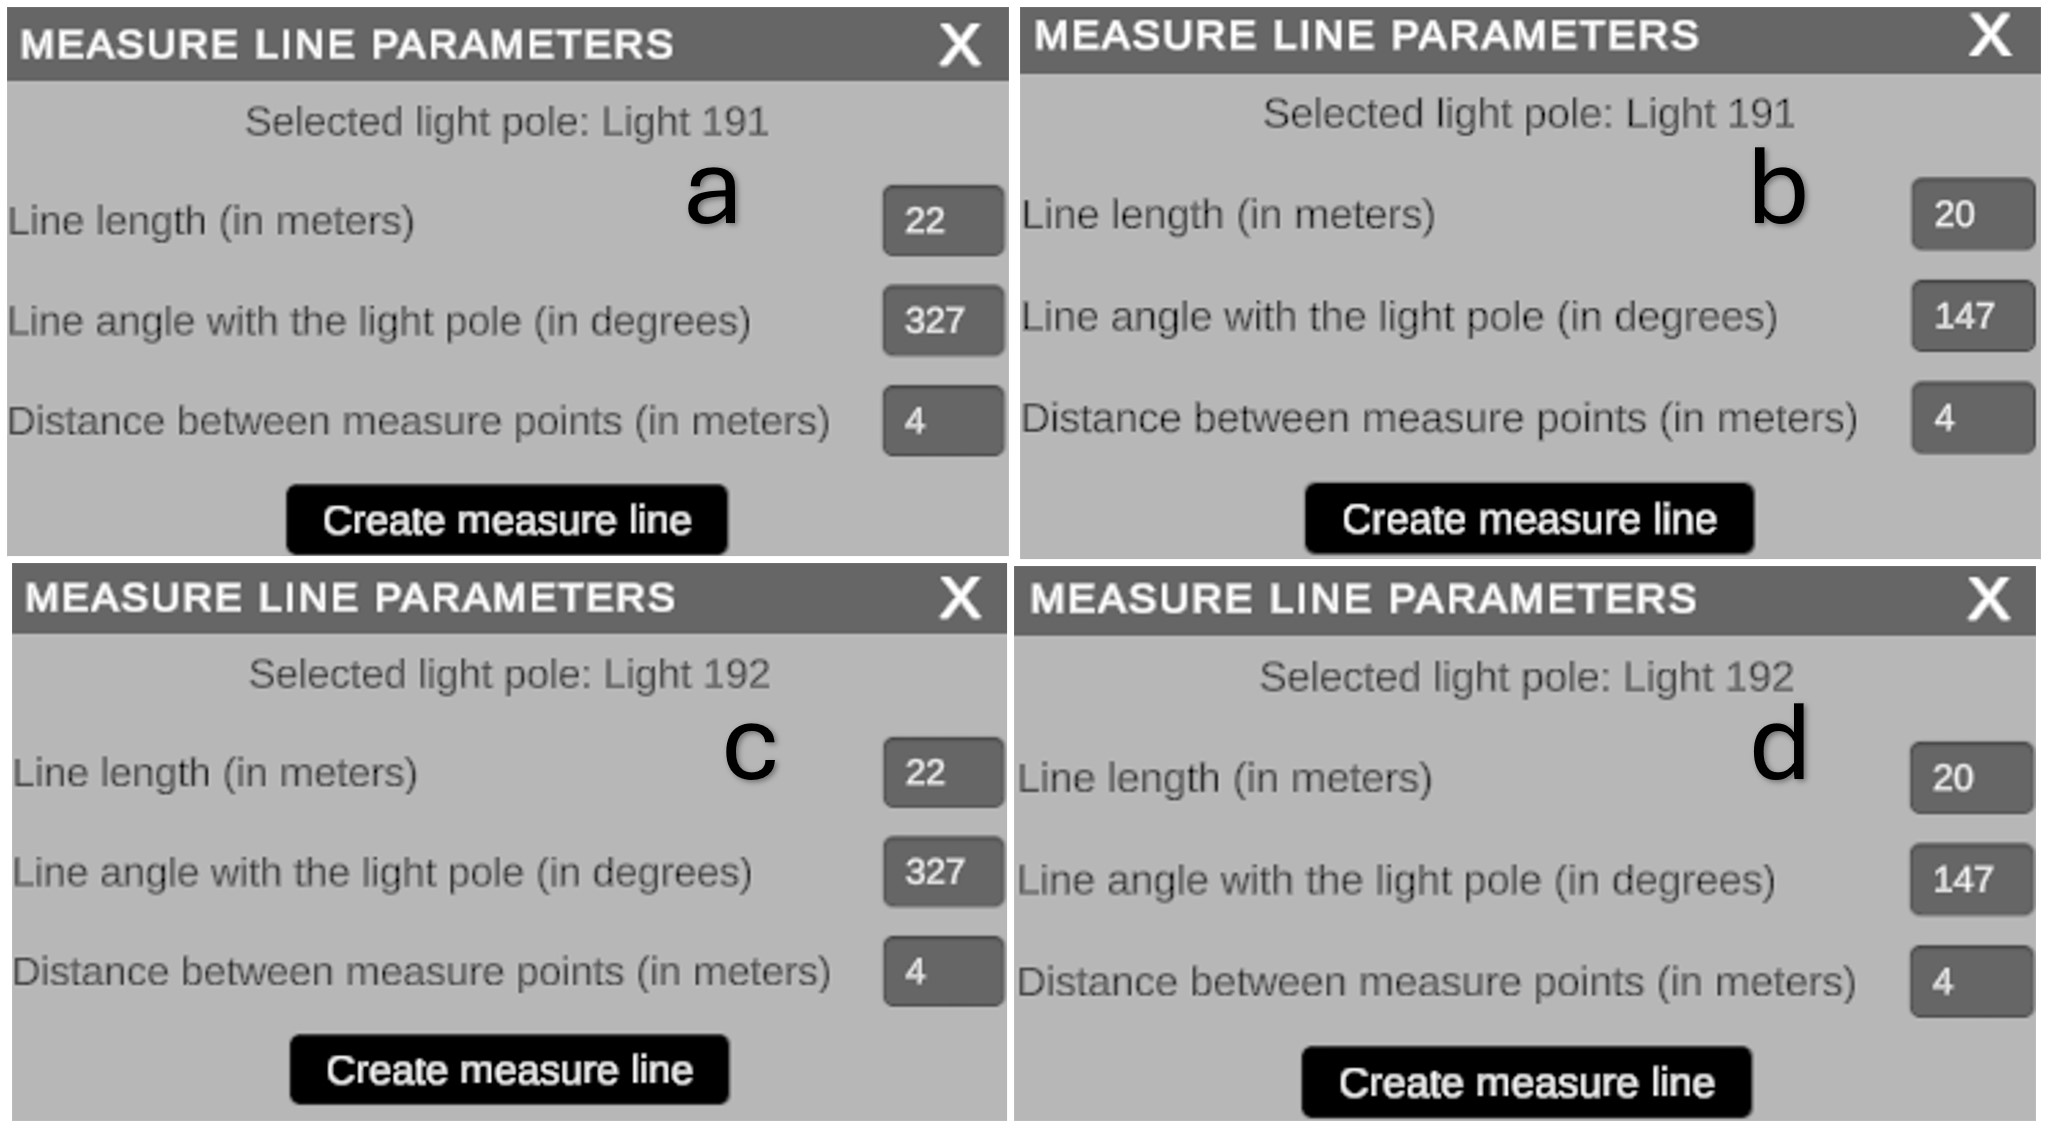
\includegraphics[width=0.8\textwidth]{Images/parameter.jpg}
    \caption[The measure line parameters for each line shown in Figure \ref{LM}]{The measure line parameters for each line shown in Figure \ref{LM}}
    \label{parameter}
\end{figure}

Another example was made for measurement points of PR9, FR5, FR10, FR15, FR20, and FR25, with different scenario. That is intervention light measurements, Scenario 1 100\% (January - snow) in Sävja, Uppsala - evening measurements - ground level (h: 0.00 m). The Geojson file is provided named case55.geojson. 
\begin{enumerate}
    \item Go to \textit{Scene} feature, change the location to Uppsala.
    \item Go to \textit{Light computation} feature, click \textit{Create measure line around light pole} button, select "light 192", and set the parameter as shown in Figure \ref{parameter}(d), then click on \textit{Create measure line}.
    \item Go to \textit{Scene} feature, set the date to 13 January 2025, the time to 18:40, the clouds to Overcast, 35\% snow.
    \item Go to \textit{Light computation} feature, check the \textit{Display graph} box to show the graph along the drawn line.
    \item Click the \textit{Import results} button, then select the case55.geojson file to import the light measurement data.
    \item if you follow all stages properly, you will get the results as shown in Figure \ref{case55}.
\end{enumerate}
\begin{figure}[H]
    \centering
    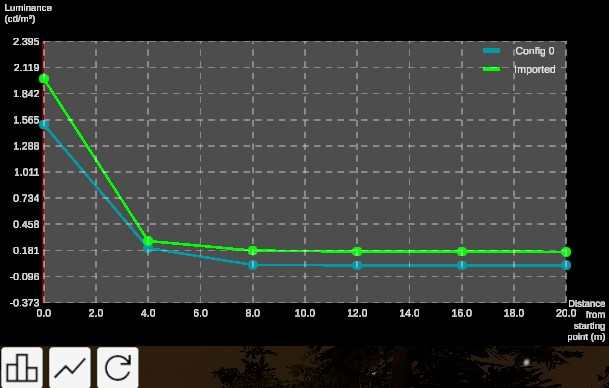
\includegraphics[width=0.8\textwidth]{Images/case55.jpg}
    \caption[The comparison of the measured data and the modelled data on PR9, FR5, FR10, FR15, FR20, and FR25, on 13 January 2025, the time to 18:40, the clouds to Overcast, 35\% snow]{The comparison of the measured data and the modelled data on PR9, FR5, FR10, FR15, FR20, and FR25, on 13 January 2025, the time to 18:40, the clouds to Overcast, 35\% snow. Blue line represents the modelled data, green line represents the measured data}
    \label{case55}
\end{figure}



%\subsection{WP6: Exploring location from local species perspective, Ålesund and Uppsala}

%by importing the text into a polygon 

%\subsection{WP6: VR protypes?}

\subsection{WP6: Survey on green space and wildlife in the neighbourhood} \label{questionnaire}

This section presents data from Work Package 6, focusing on residents' opinions about their neighbourhood. The information was gathered through a questionnaire answered by local residents, addressing topics such as green spaces, wildlife, and vegetation in the area. Responses were categorized into five levels: strongly agree, agree, neutral, disagree, and strongly disagree. The questions are listed below:
\begin{itemize}
    \item There should be more green space in my neighbourhood
    \item The green space in my neighbourhood is very important to me.  
    \item I know a lot about the wild plants in my neighbourhood. 
    \item I know a lot about the wild animals in my neighbourhood. 
    \item Urban animals and plants have as much right as humans to exist.     
\end{itemize}
To visualize the questionnaire data, two display options are available: (i) using the five responses as variables, or (ii) using the five questions as variables.

The first option is useful for identifying which questions received the most "strongly agree," "neutral," or "strongly disagree" responses. To visualize this data, use the provided GeoJSON file named Arne\_questionnaire\_opinion.geojson and follow these steps within the software:
\begin{itemize}
    \item Go to \textit{Data visualization} feature.
    \item Click the \textit{Add dataset} button, and select the file "Arne\_questionnaire\_opinion.geojson"
    \item Zoom out/in and adjust the camera to find the analyzed path
\end{itemize}
Figure \ref{agree} illustrates the results, where the listed variables are strongly agree, agree, neutral, disagree, and strongly disagree. In this context, (1) represents the opinion that "there should be more green space in my neighbourhood." (2) corresponds to the opinion that "the green space in my neighbourhood is very important to me." (3) reflects the opinion that "I know a lot about the wild plants in my neighbourhood." (4) relates to the opinion that "I know a lot about the wild animals in my neighbourhood." (5) expresses the opinion that "urban animals and plants have as much right as humans to exist." Part (b) of Figure \ref{agree} indicates that local residents are most likely to feel neutral towards the idea of making the neighbourhood greener and their knowledge of wild plants. Part (c) of Figure \ref{agree} shows that residents strongly agree on the importance of green space and equal rights for all living beings. Part (d) of Figure \ref{agree} reveals that only a small number of respondents strongly disagree with any of the questions.
\begin{figure}[H]
    \centering
    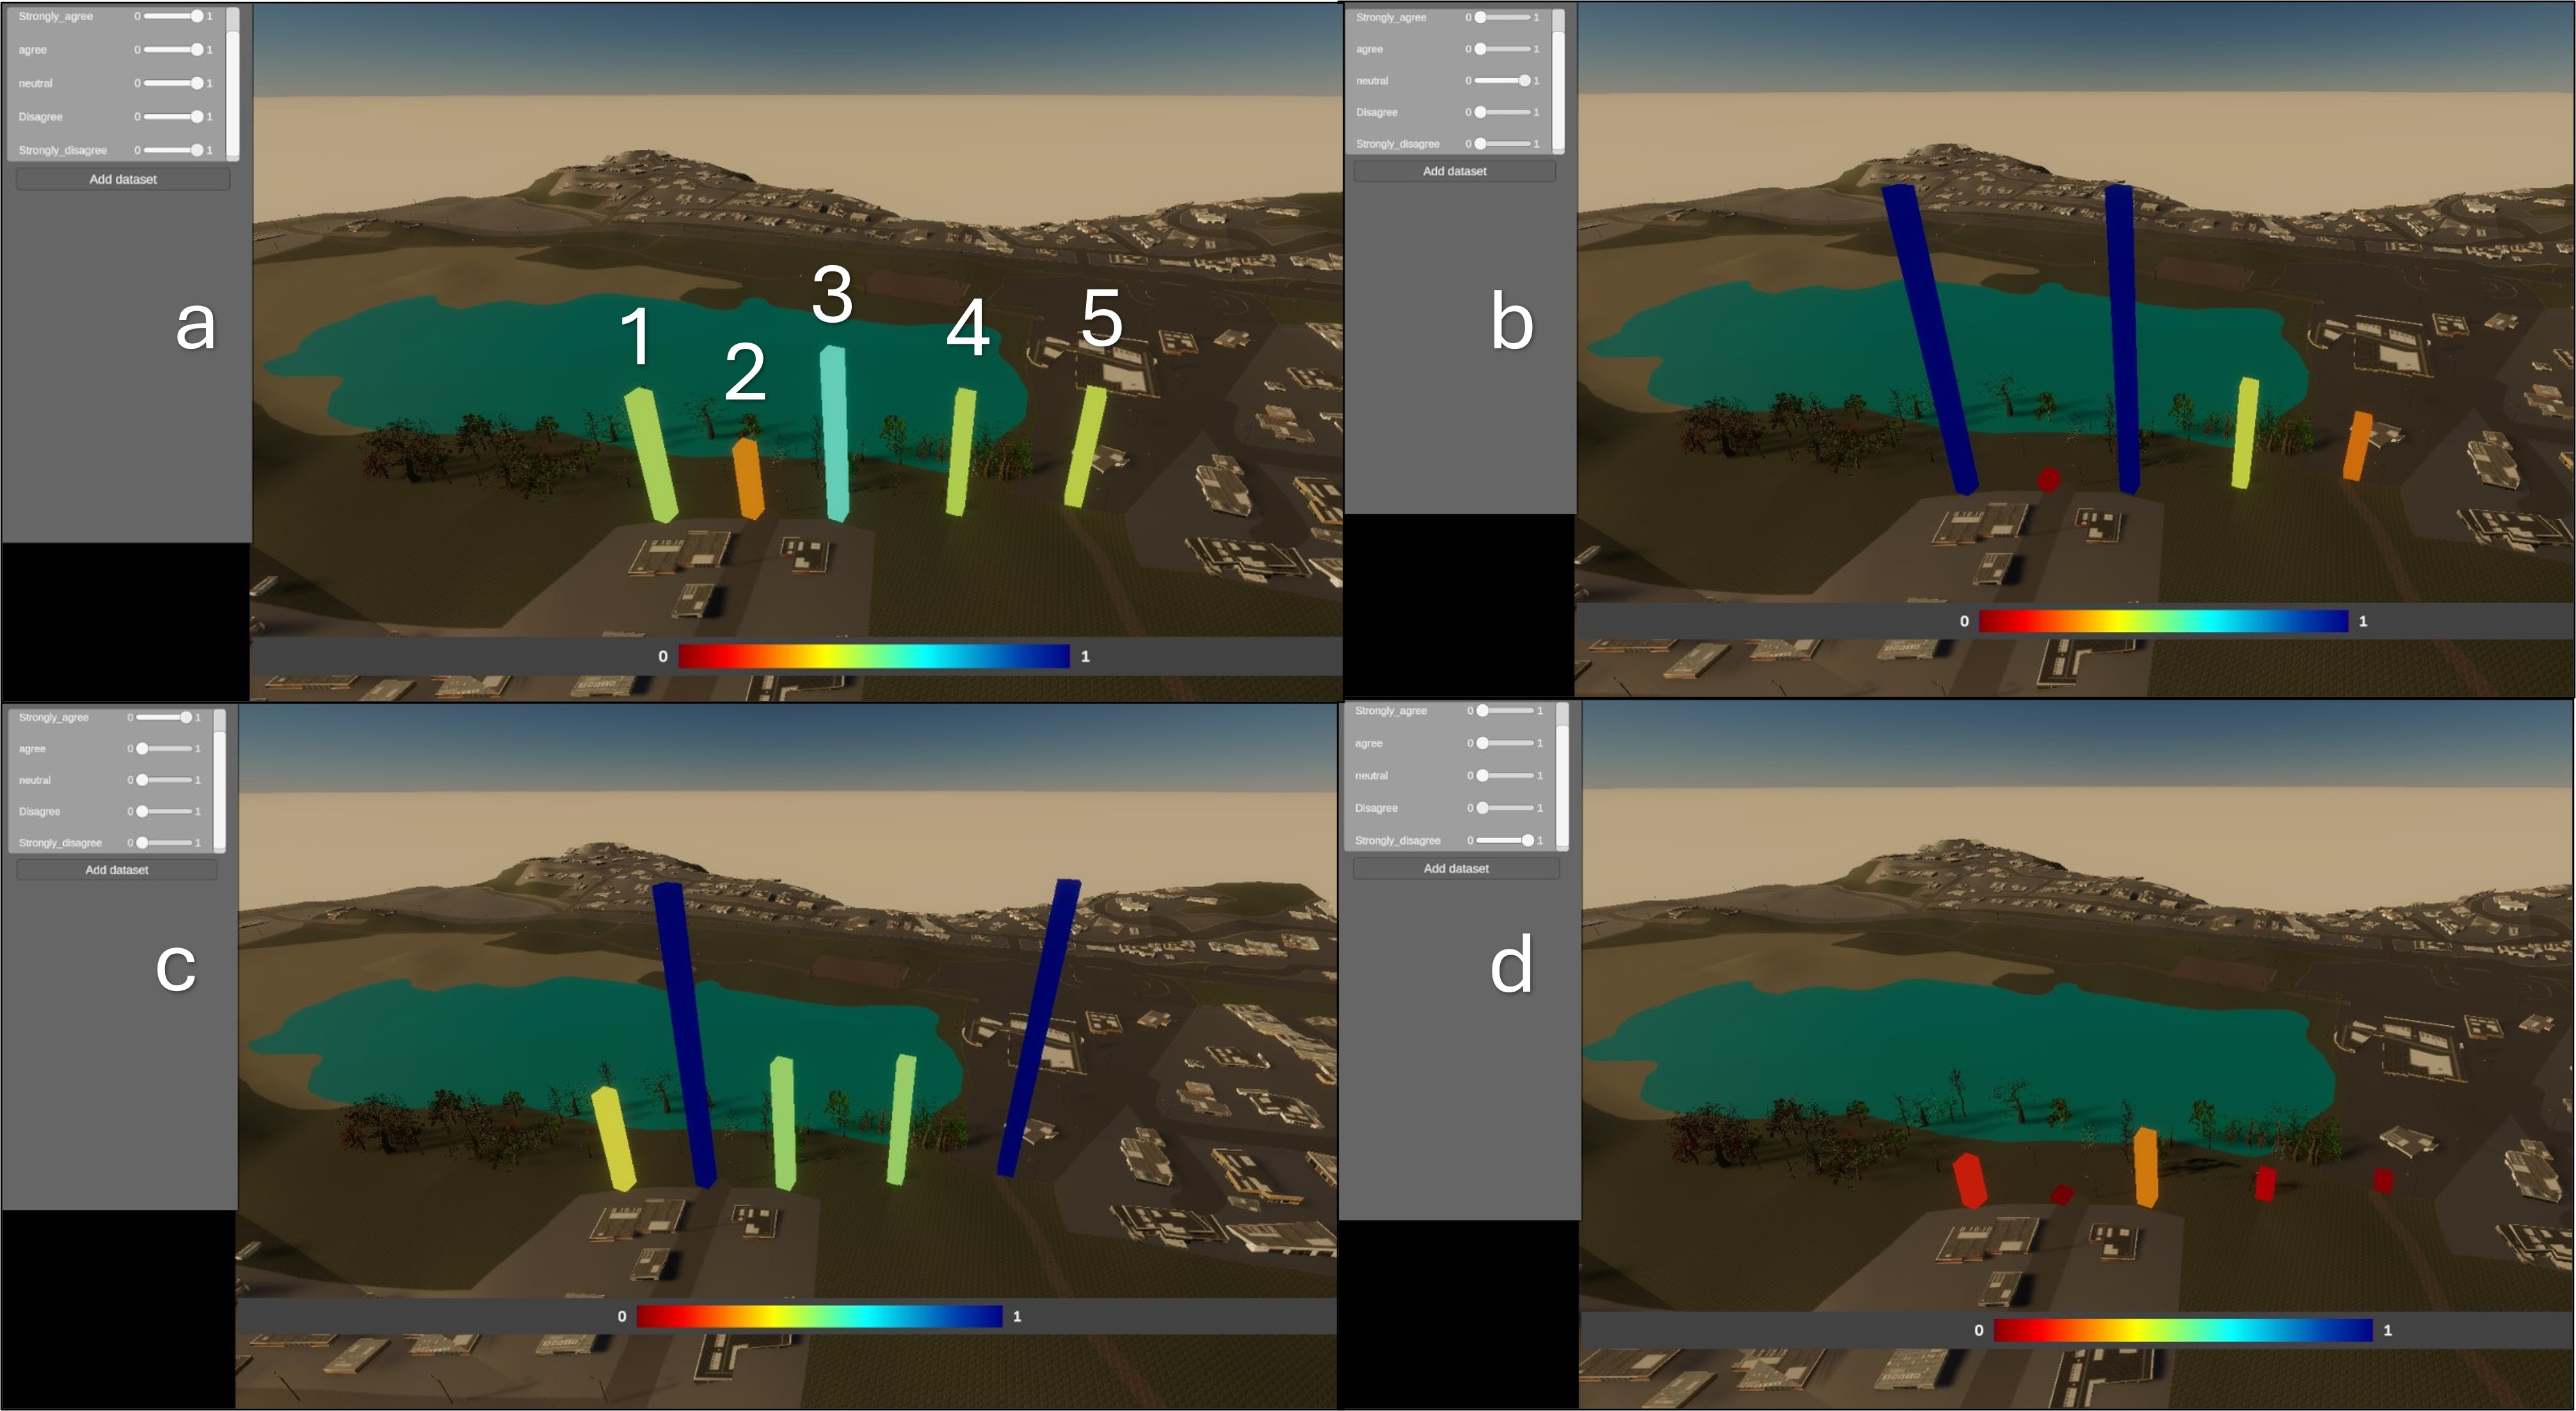
\includegraphics[width=0.9\textwidth]{Images/agree.jpg}
    \caption[The first option to visualize the questionnaire information, where the five answers as the listed variables]{The first option to visualize the questionnaire information, where the five answers as the listed variables. (a) all answers are considered. (b) only the neutral answer is considered. (c) only the strongly agree answer is considered. (d) only the strongly disagree answer is considered.}
    \label{agree}
\end{figure}

The second option is useful for viewing residents’ responses to each individual question. To visualize this data, use the GeoJSON file named Arne\_questionnaire\_5var.geojson and follow these steps in the software:
\begin{itemize}
    \item Go to \textit{Data visualization} feature.
    \item Click the \textit{Add dataset} button, and select the file "Arne\_questionnaire\_5var.geojson"
    \item Zoom out/in and adjust the camera to find the analyzed path
\end{itemize}
Figure \ref{greener} displays the results, where the listed variables correspond to the numbers (1) through (5) from Figure \ref{agree}, and are shortened as greener, green\_importance, wild\_plants, wild\_animals, and equal\_right. In Figure \ref{greener}, (1) represents the answer "strong agree", (2) represents "agree", (3) represents "neutral", (4) represents "disagree", and (5) represents "strong disagree".
Part (a) of Figure \ref{greener} indicates that residents generally agree with all the questions.
Part (b) highlights that residents tend to feel neutral about the idea of making the area greener.
Part (f) shows that residents strongly agree with the concept of equal rights among urban animals, plants, and humans.
\begin{figure}[H]
    \centering
    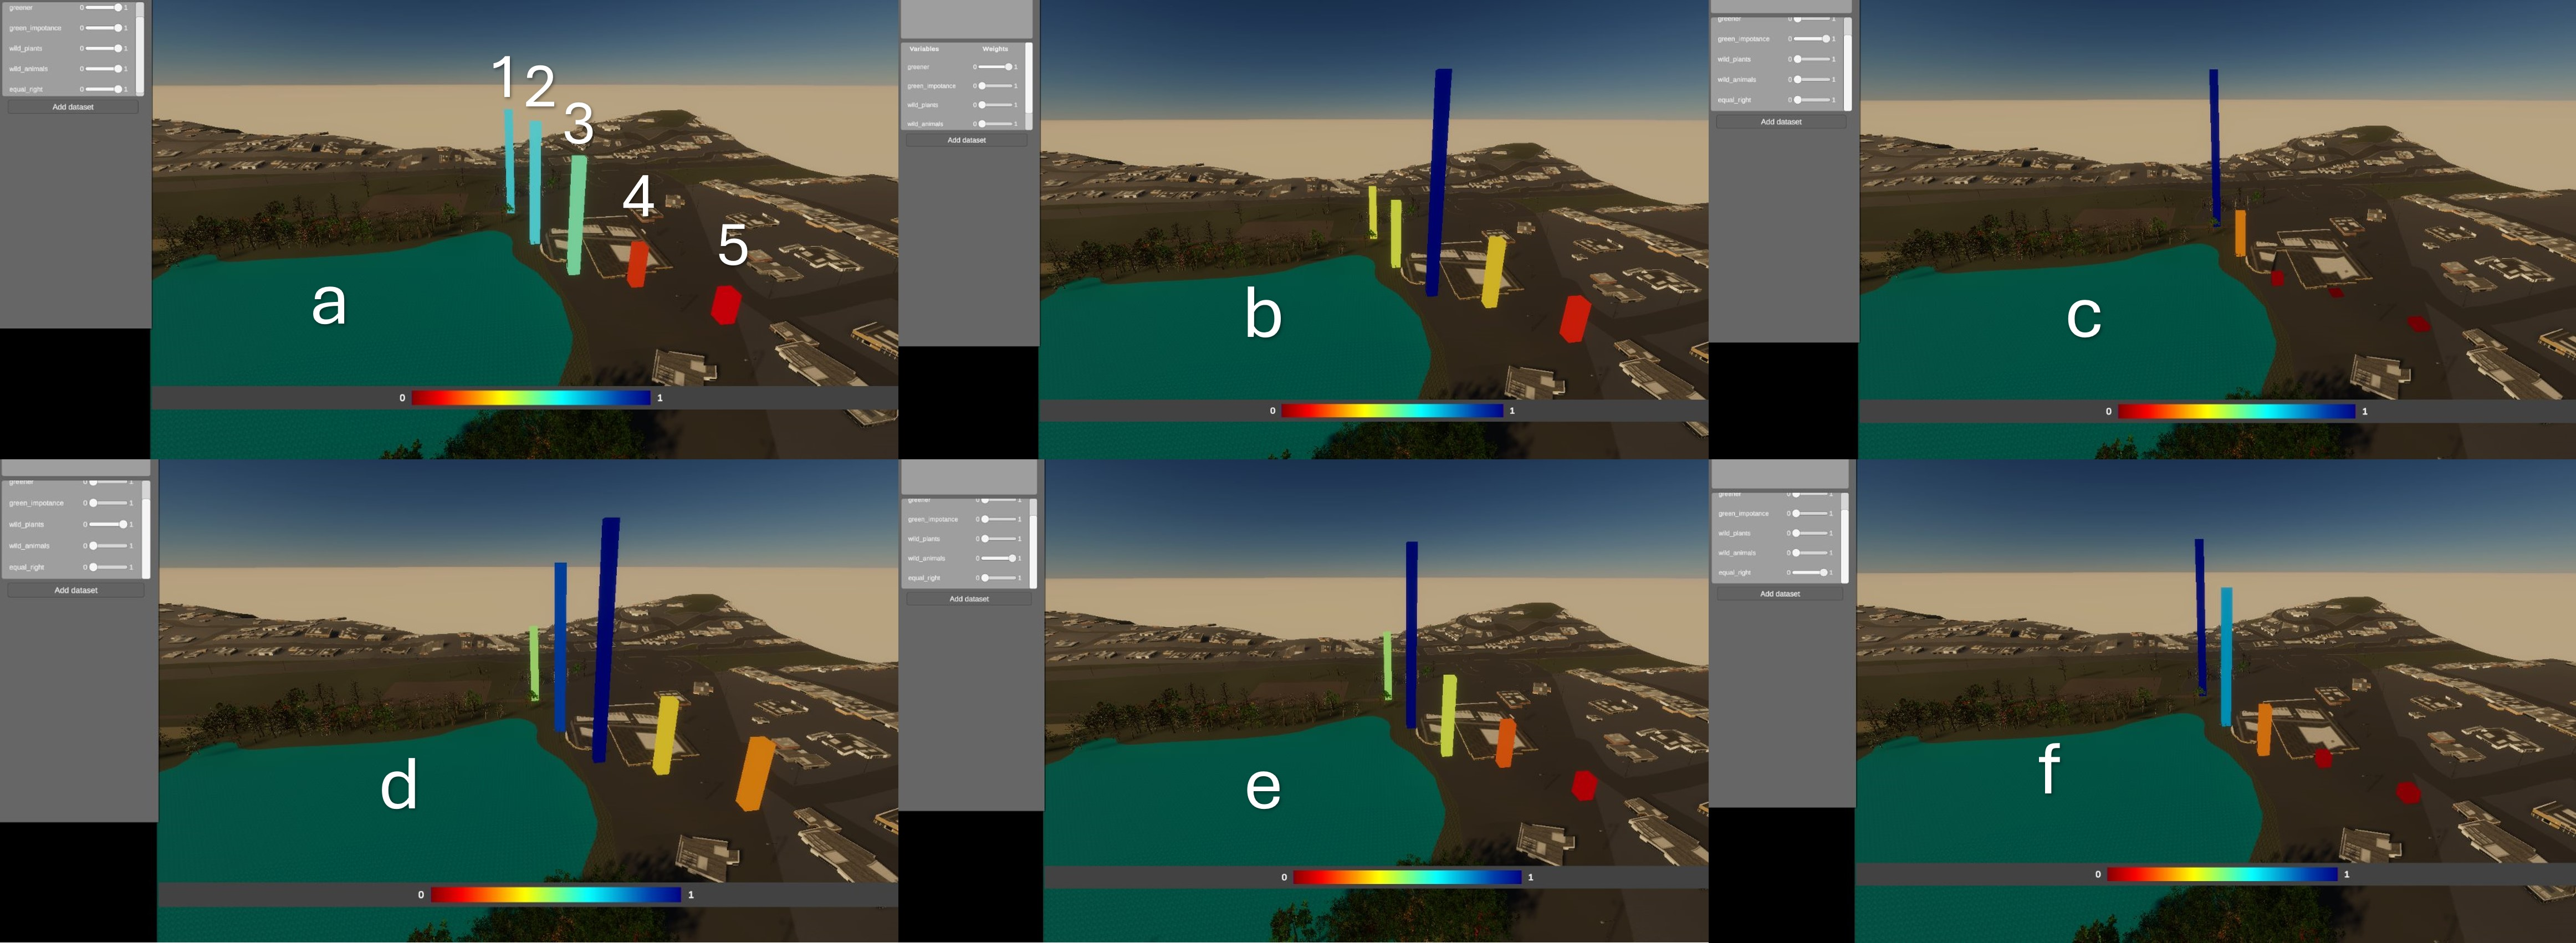
\includegraphics[width=1\textwidth]{Images/greener.jpg}
    \caption[The second option to visualize the questionnaire information, where the five questions as the listed variables]{The second option to visualize the questionnaire information, where the five questions as the listed variables. (a) all questions are considered. (b) only the greener question is considered. (c) only the question regarding the importance of green space is considered. (d) only the question regarding the knowledge of wild plants is considered. (e) only the question regarding the knowledge of wild animals is considered. (f) only the question regarding the equal right over all living things is considered.}
    \label{greener}
\end{figure}

\subsection{WP6: Urban lifestyle vs wildlife protection} \label{urban}

On the questionnaire, an additional question was included to explore residents’ views on the balance between a comfortable urban lifestyle and wildlife protection. The question was stated as: \textbf{How do you think about wildlife protection and urban lifestyle?} with the following response options: 
\begin{itemize}
    \item To protect urban wildlife and plants I have to accept restrictions in my lifestyle
    \item Protecting urban wildlife and plants is important, but not if it means changing my lifestyle
    \item To enjoy a pleasant and comfortable lifestyle, I can’t avoid losing urban wildlife and plants
\end{itemize}
To visualize this data using the data visualization feature, a GeoJSON file named lifestyle\_wildlife.geojson is provided. Follow these steps in the software: 
\begin{itemize}
    \item Go to \textit{Data visualization} feature.
    \item Click the \textit{Add dataset} button, and select the file "lifestyle\_wildlife.geojson"
    \item Zoom out/in and adjust the camera to find the analyzed path
\end{itemize}

Figure \ref{how} illustrates local residents' responses regarding their views on wildlife protection and urban lifestyle. The variables were defined based on the available response options. \textbf{wildlife\&plants} refers to residents who prioritize urban wildlife and plants over their own lifestyle, expressing a willingness to accept lifestyle restrictions to support conservation. \textbf{both} represents those who believe protecting urban wildlife and plants is important—but not at the cost of changing their lifestyle. \textbf{lifestyle} reflects residents who prioritize a pleasant and comfortable lifestyle, even if it results in the loss of urban wildlife and plants.
\begin{figure}[H]
    \centering
    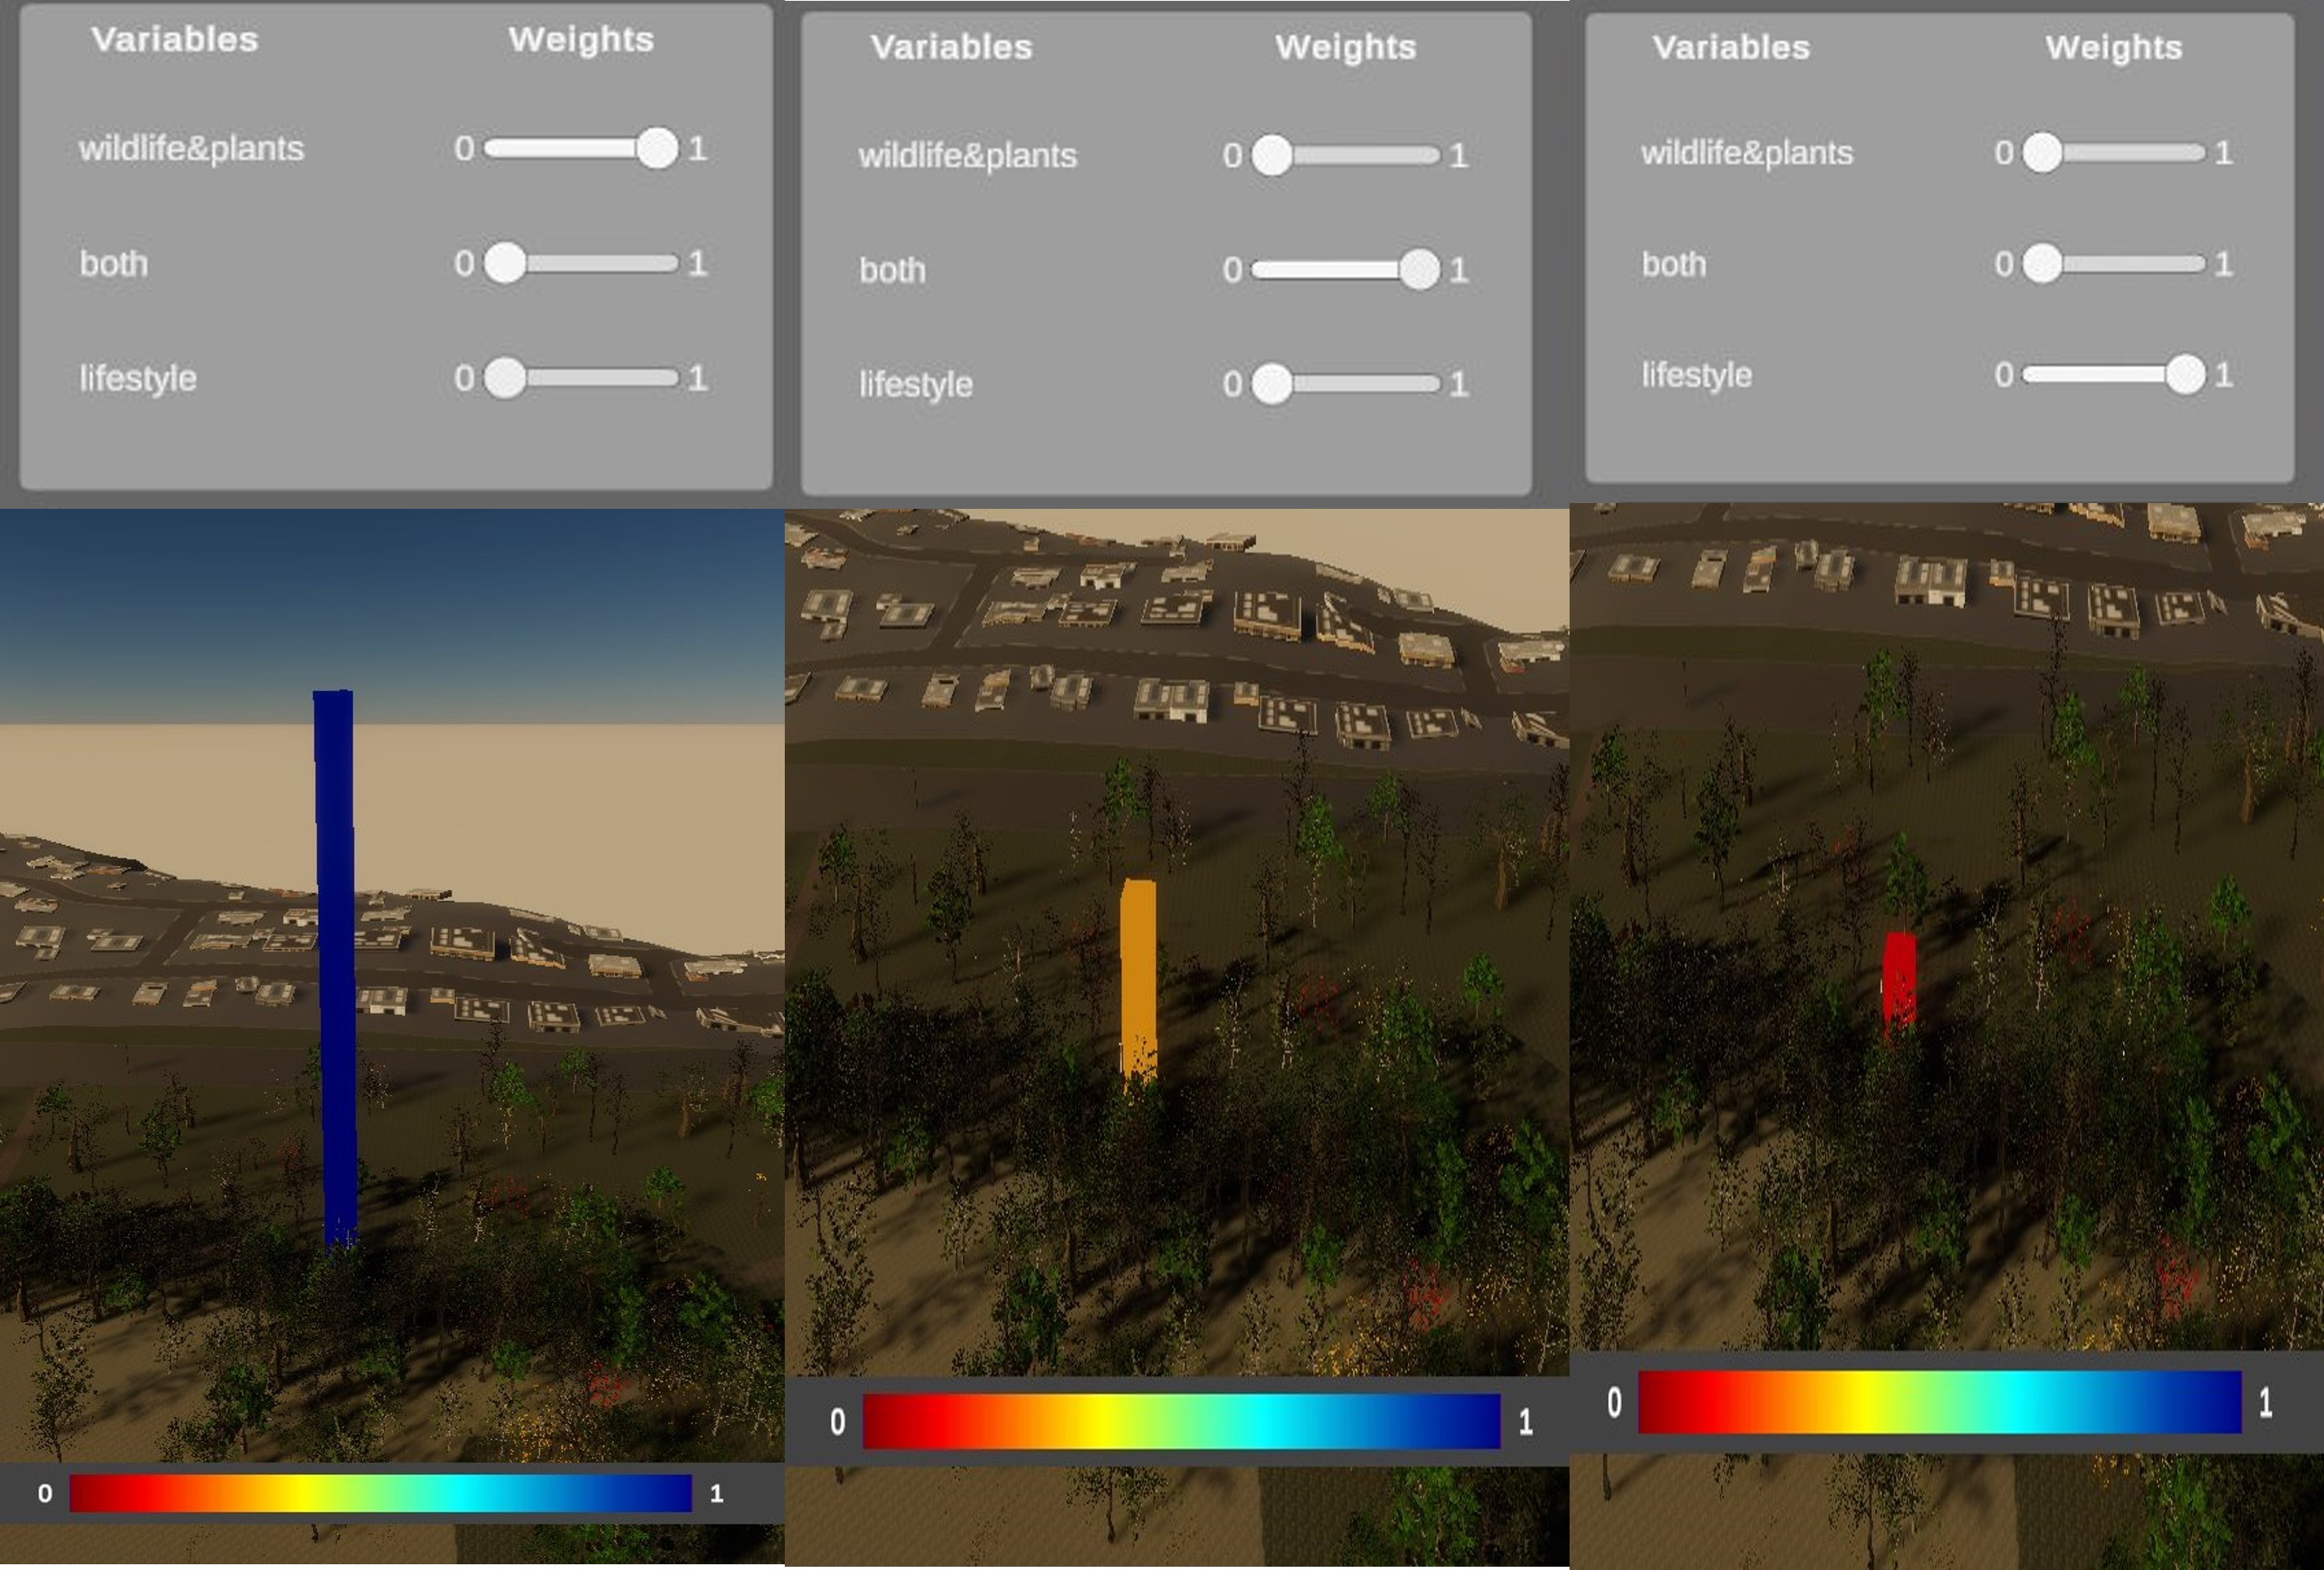
\includegraphics[width=0.7\textwidth]{Images/how.jpg}
    \caption[The questionnaire answer of how local residents think about wildlife protection and urban lifestyle]{The questionnaire answer of how local residents think about wildlife protection and urban lifestyle.}
    \label{how}
\end{figure}